\documentclass[table]{beamer}
%[]中可以使用handout、trancompress等参数

%指定package
\usepackage{subfigure}
\usepackage{manfnt}%%% Dangerous Bend Symbols}\dbend \lhdbend \reversedvideodbend \textdbend \textlhdbend
\usepackage{multicol}
\usepackage{bbding}% 手势 \HandRight \HandLeft %\FiveStar \FourStar \SixStar
\usepackage{wasysym}
\usepackage{wasysym}
\usepackage{mflogo}

%指定beamer的模式与主题
\mode<presentation>
{
  \usetheme{CambridgeUS}
%Good themes
%\usetheme{CambridgeUS}
%\usetheme{Antibes}
%\usetheme{Madrid}
%\usetheme{Berkeley}
%\usetheme{Boadilla}

%\usecolortheme{default}
%\usecolortheme{orchid}
%\usecolortheme{whale}
\usecolortheme{spruce}
%\usefonttheme{professionalfonts}
}

%这里还可以选择别的主题:Bergen, Boadilla, Madrid, AnnArbor, CambridgeUS, Pittsburgh, Rochester, Warsaw, ...
%有导航栏的Antibes, JuanLesPins, Montpellier, ...
%有内容的Berkeley, PaloAlto, Goettingen, Marburg, Hannover, ...
%有最小导航栏的Berlin, Ilmenau, Dresden, Darmstadt, Frankfurt, Singapore, Szeged, ...
%有章和节表单的Copenhagen, Luebeck, Malmoe, Warsaw, ...

%\usecolortheme{default}
%设置内部颜色主题(这些主题一般改变block里的颜色);这个主题一般选择动物来命名
%这里还可以选择别的颜色主题,如默认的和有特别目的的颜色主题default,structure,sidebartab,全颜色主题albatross,beetle,crane,dove,fly,seagull,wolverine,beaver

%\usecolortheme{orchid}
%设置外部颜色主题(这些主题一般改变title里的颜色);这个主题一般选择植物来命名
%这里还可以选择别的颜色主题,如默认的和有特别目的的颜色主题lily,orchid,rose

%\usecolortheme{whale}
%设置字体主题;这个主题一般选择海洋动物来命名
%这里还可以选择别的颜色主题,如默认的和有特别目的的颜色主题whale,seahorse,dolphin

%\usefonttheme{professionalfonts}
%类似的还可以定义structurebold,structuresmallcapsserif,professionalfonts


% 控制 beamer 的风格,可以根据自己的爱好修改
%\usepackage{beamerthemesplit} %使用 split 风格
%\usepackage{beamerthemeshadow} %使用 shadow 风格
%\usepackage[width=2cm,dark,tab]{beamerthemesidebar}


% 设定英文字体
\usepackage{fontspec}
\usepackage{ listings}
\setmainfont{DejaVu Sans}
%\setmainfont{Times New Roman}
%\setsansfont{Arial}
%\setmonofont{Courier New}

% 设定中文字体
\usepackage[BoldFont,SlantFont,CJKchecksingle,CJKnumber]{xeCJK}
%\setCJKmainfont[BoldFont={Adobe Heiti Std},ItalicFont={Adobe Kaiti Std}]{Adobe Song Std}
\setCJKmainfont[BoldFont={WenQuanYi Micro Hei},ItalicFont={WenQuanYi Micro Hei}]{WenQuanYi Micro Hei}
\setCJKsansfont{WenQuanYi Micro Hei}
\setCJKmonofont{WenQuanYi Micro Hei}
\punctstyle{hangmobanjiao}

\defaultfontfeatures{Mapping=tex-text}
\usepackage{xunicode}
\usepackage{xltxtra}

\XeTeXlinebreaklocale "zh"
\XeTeXlinebreakskip = 0pt plus 1pt minus 0.1pt

\usepackage{setspace}
\usepackage{booktabs}
\usepackage{colortbl,xcolor}
\usepackage{hyperref}
%\hypersetup{xetex,bookmarksnumbered=true,bookmarksopen=true,pdfborder=1,breaklinks,colorlinks,linkcolor=blue,filecolor=black,urlcolor=cyan,citecolor=green}
\hypersetup{xetex,bookmarksnumbered=true,bookmarksopen=true,pdfborder=1,breaklinks,colorlinks,linkcolor=cyan,filecolor=black,urlcolor=blue,citecolor=green}

% 插入图片
\usepackage{graphicx}
% 指定存储图片的路径(当前目录下的figures文件夹)
\graphicspath{{figures/}}

% 可能用到的包
\usepackage{amsmath,amssymb}
\usepackage{multimedia}
\usepackage{multicol}

% 定义一些自选的模板,包括背景、图标、导航条和页脚等,修改要慎重
% 设置背景渐变由10%的红变成10%的结构颜色
%\beamertemplateshadingbackground{red!10}{structure!10}
%\beamertemplatesolidbackgroundcolor{white!90!blue}
% 使所有隐藏的文本完全透明、动态,而且动态的范围很小
\beamertemplatetransparentcovereddynamic
% 使itemize环境中变成小球,这是一种视觉效果
\beamertemplateballitem
% 为所有已编号的部分设置一个章节目录,并且编号显示成小球
\beamertemplatenumberedballsectiontoc
% 将每一页的要素的要素名设成加粗字体
\beamertemplateboldpartpage

% item逐步显示时,使已经出现的item、正在显示的item、将要出现的item呈现不同颜色
\def\hilite<#1>{
 \temporal<#1>{\color{gray}}{\color{blue}}
    {\color{blue!25}}
}

% 自定义彩色块状结构的颜色
\setbeamercolor{bluecyanbgcolor}{fg=blue,bg=cyan}
\setbeamercolor{redblackbgcolor}{fg=red,bg=black}
\setbeamercolor{greenwhitebgcolor}{fg=green,bg=white}
\setbeamercolor{blueblackbgcolor}{fg=blue,bg=black}
\setbeamercolor{yellowmagentabgcolor}{fg=yellow,bg=green}
\setbeamercolor{blackorangebgcolor}{fg=black,bg=orange}
\setbeamercolor{magentabgcolor}{fg=,bg=magenta}



% 在表格、图片等得标题中显示编号
\setbeamertemplate{caption}[numbered]

% 打开PDF后直接全屏
\hypersetup{pdfpagemode={FullScreen}}


% 使用 \part,\section,\subsection,subsubsection 等命令组织文档结构
% 使用 \frame 命令制作幻灯片

\begin{document}

\logo{
\includegraphics[height=0.09\textwidth]{redhat.jpg}}
\title[GNU Emacs]{GNU Emacs}
\author[lkong]{Lingfei Kong}
\institute[RedHat]{lkong@redhat.com}
\date{\today}

% 定义目录页
\AtBeginPart{
  \frame{
    \frametitle{\partpage}
    \begin{multicols}{2}
% 如果目录过长,可以打开这个选项分两栏显示
      \tableofcontents
% 使用这个命令自动生成目录
    \end{multicols}
  }
}

%\AtBeginSsection[]
%{
%  \begin{frame}<beamer>
%    \frametitle{Agenda}
%	\setcounter{tocdepth}{2}
%    \tableofcontents[currentsection,currentsubsection]
%  \end{frame}
%}

% 在每个Section前都会加入的Frame
\AtBeginSection[]
{
  \begin{frame}<beamer>
    \frametitle{Agenda}
    \begin{multicols}{2}
	\setcounter{tocdepth}{1}
    \tableofcontents[currentsection]
    \end{multicols}
  \end{frame}
}
% 在每个Subsection前都会加入的Frame
\AtBeginSubsection[]
{
  \begin{frame}<beamer>
%\begin{frame}<handout:0>
% handout:0 表示只在手稿中出现
    \frametitle{Agenda}
    \begin{multicols}{2}
	\setcounter{tocdepth}{2}
    \tableofcontents[currentsection,currentsubsection]
    \end{multicols}
% 显示在目录中加亮的当前章节
  \end{frame}
}

\iffalse
\AtBeginSubsubsection[]
{
  \begin{frame}<beamer>
%\begin{frame}<handout:0>
% handout:0 表示只在手稿中出现
    \frametitle{Agenda}
    \begin{multicols}{2}
	\setcounter{tocdepth}{3}
    \tableofcontents[currentsection,currentsubsection]
    \end{multicols}
% 显示在目录中加亮的当前章节
  \end{frame}
}
\fi

%\theoremstyle{block}
%\newtheorem{EK}{Emacs Key}
%\theoremstyle{definition}
%\newtheorem{EC}{Emacs Configure}
%\theoremstyle{example}
%\newtheorem{IP}{Install Packages}

\defverbatim[colored]\etags{%
\begin{lstlisting}[frame=single, emph={find}, emphstyle={\color{blue}}]
find . -name "*.py" -print | etags -
\end{lstlisting}
}


\begin{frame}
  \titlepage
\end{frame}

\begin{frame}[plain]
  \frametitle{Agenda}
  \setcounter{tocdepth}{2}
  \tableofcontents
\end{frame}

\section{Author}
\begin{frame}
	\frametitle{Richard Stallman}
	\begin{figure}[htbp]
    \centering
    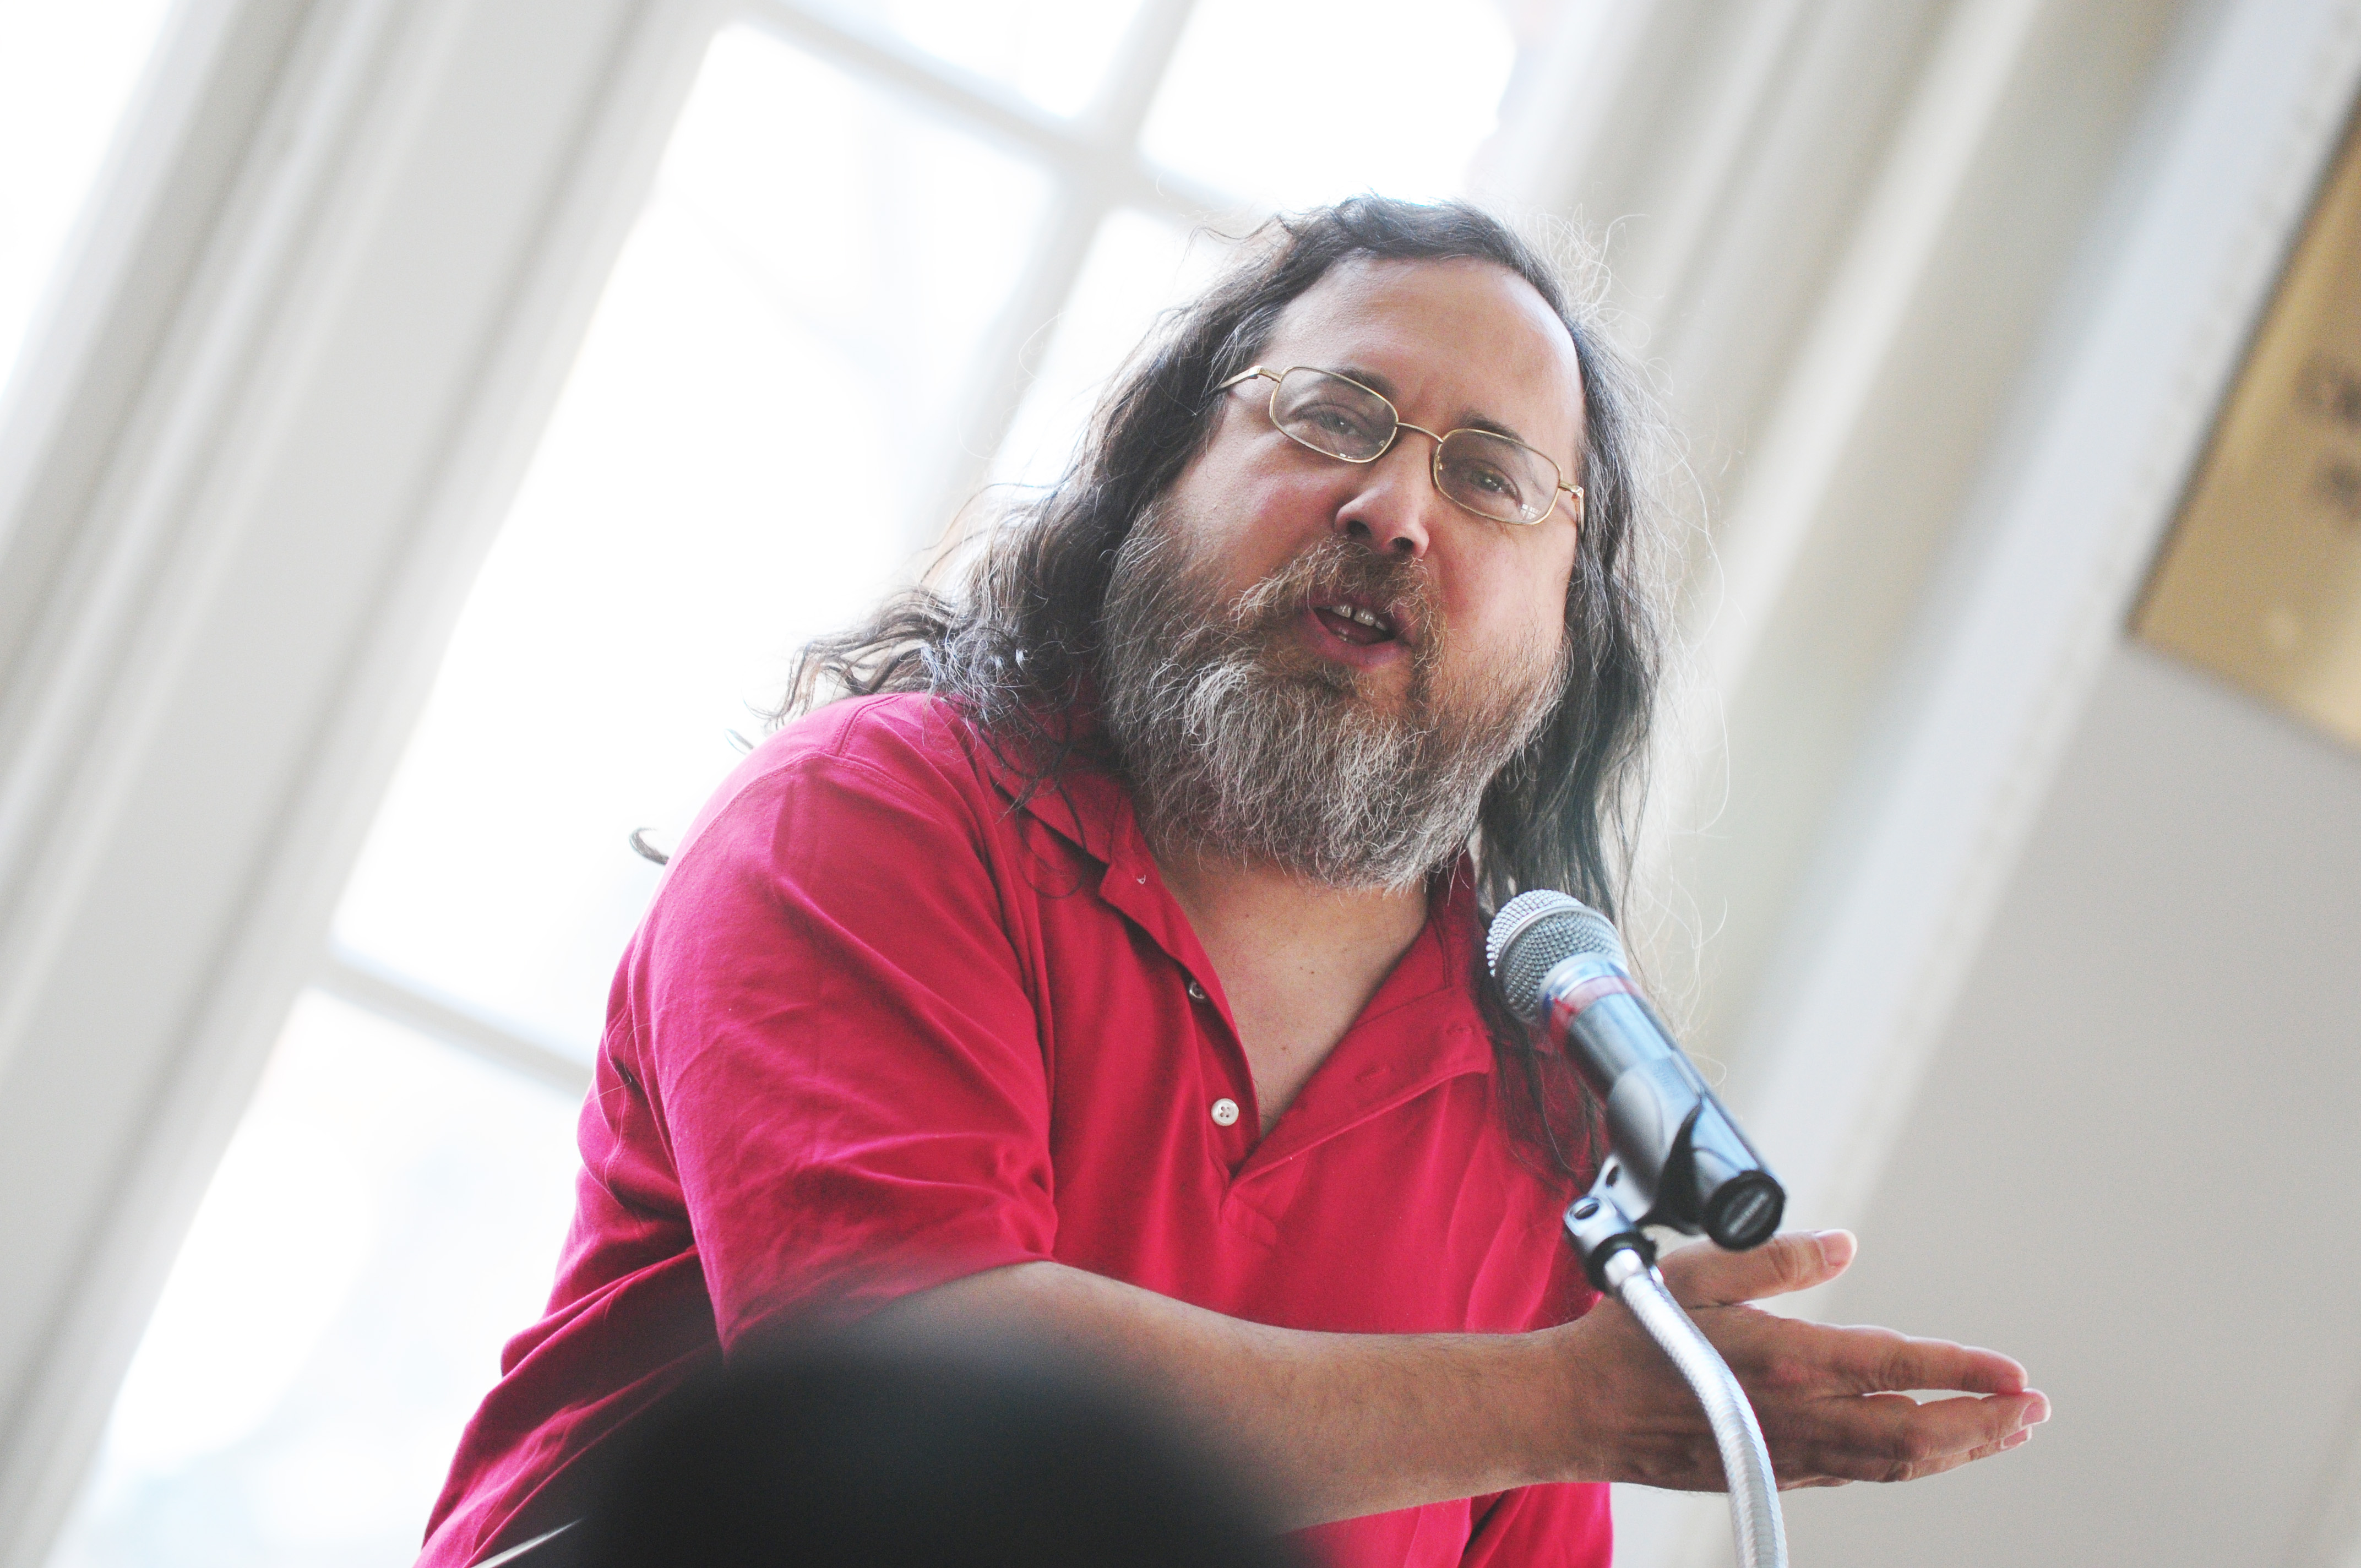
\includegraphics[width=8cm]{rich.jpg}
    \caption{Richard Stallman}
    \label{fig:power}
    \end{figure}
\end{frame}
\section{Why Emacs}
\begin{frame}
    \begin{itemize}[<+-|alert@+>]
        \hilite <1> \item Org-mode
        \hilite <2> \item Buffer management, very fast when switch buffers or files
        \hilite <3> \item Have very powerful features
        \hilite <4> \item Can do many things in one emacs session
        \hilite <5> \item Directory Editor
        \hilite <6> \item Bookmark management
        \hilite <7> \item Can configure as a IDE (Python \& C \& Other language)
    \end{itemize}
\end{frame}
\section{Emacs Basic Features}
\subsection{Key introduce}
\begin{frame}
	\frametitle{Key introduce}
	\begin{block}{Emacs Key}
    C = Control\\
    M = Alt = Esc\\
    Del = Backspace
	\end{block}
	\pause
	\begin{exampleblock}{Emacs Configure}
    \~/.emacs\\
    \~/.emacs.d
	\end{exampleblock}
	\pause
	\begin{alertblock}{Install Packages}
    M-x package-list-packages
	\end{alertblock}
\end{frame}
\subsection{As a editor}
\subsubsection{Open, Save, Save as, Close file, Exit emacs}
\begin{frame}[allowframebreaks]
\frametitle{Open, Save, Save as, Close file, Exit emacs}
    \begin{itemize}
        \item C-x C-f: Visit a file ('find-file').
        \item C-x C-r: Visit a file for viewing, without allowing changes to it ('find-file-read-only').
        \item C-x C-v: Visit a different file instead of the one visited last
        \item C-x C-s: Save the current buffer to its file ('save-buffer').
        \item C-x s: Save any or all buffers to their files ('save-some-buffers').
        \item C-x C-w: Save the current buffer with a specified file name ('write-file').
        \item C-x C-c: Offer to save each buffer, then kill the current connection. If the current frame has no client, kill Emacs itself.
        \item C-x i: Insert contents of file FILENAME into buffer after point. Set mark after the inserted text.
        \item C-x b: Display buffer BUFFER-OR-NAME in the selected window.
        \item C-x C-b: Display a list of existing buffers.
        \item C-x k: Kill the current buffer.
    \end{itemize}
\end{frame}
\subsubsection{Buffer}
\begin{frame}
\frametitle{Buffer}
    \begin{itemize}
        \item C-x <LEFT> , C-x <RIGHT>
        \item M-x rename-buffer
        \item C-x C-b:

  . in the first field of a line indicates that the buffer is current. \% indicates a read-only buffer. \* indicates that the buffer is “modified”.

  d: Flag the buffer for deletion (killing)

  s: Flag the buffer for saving (Buffer-menu-save)

  x: Perform all flagged deletions and saves

  u: Remove all flags from the current line, and move down

  f/ENTER: Select this line's buffer in this window.

  q: Quit buffer list

  T: Delete, or reinsert, lines for non-file buffers Buffer-menu-toggle-files-only)
    \end{itemize}
\end{frame}
\subsubsection{Move cource}
\begin{frame}
\frametitle{Move course}
    \begin{itemize}
        \item C-f, C-b, C-p, C-n: forward; backward; previous line; next line
        \item M-f, M-b: forward word; backward word
        \item C-a, C-e: Go to the beginning of the line; Go to the end of the line.
        \item C-v, M-v: Scroll text of selected window upward ARG lines; Scroll text of selected window down ARG line
        \item M-<, M->: Move point to the beginning of the buffer; Move point to the end of the buffer
    \end{itemize}
\end{frame}
\subsubsection{Editing}
\begin{frame}[allowframebreaks]
\frametitle{Editing}
    \begin{itemize}
        \item M-n: Repeat n times for the next command
        \item M-d: Kill characters forward until encountering the end of a word
        \item C-d: Delete the next character
        \item C-k: Kill line, to tags or end of line.
        \item C-Space/C-@: Set the mark at point, and activate it.
        \item C-w: Kill ("cut") text between point and mark.
        \item M-w: Save the region as if killed, but don't kill it.
        \item C-j: Goto next table row or insert a newline and indent.
        \item C-y: Yank.  If the kill is a subtree, treat it specially.
        \item M-y: Replace just-yanked stretch of killed text with a different stretch.
        \item C-x C-x: Put the mark where point is now, and point where the mark is now.
        \item C-t, M-t: Interchange characters around point, moving forward one character; Interchange words around point, moving forward one word.
        \item M-u, M-l, M-c: Convert word to upper case; Convert word to upper case; Convert word to lower case; Capitalize word
    \end{itemize}
\end{frame}
\subsubsection{Search and Replace}
\begin{frame}
\frametitle{Search and Replace}
    \begin{itemize}
        \item C-s, C-r: Search forward; Search backword
        \item M-\%: Query and replace

        .: only replace the current place and exit

        !: replace all place

        q: exit
        \item Find more at \href{http://kongll.github.io/2014/10/30/Emacs-keys/}{\beamerbutton{Emacs Keys}}
    \end{itemize}
\end{frame}
\subsubsection{Windows}
\begin{frame}
\frametitle{Windows}
    \begin{itemize}
        \item C-x 2: Split the selected window into two windows, one above the other
        \item C-x 3: Split the selected window into two side-by-side windows
        \item C-x o: Select another window in cyclic ordering of windows.
        \item C-x 0: Delete WINDOW.
        \item C-x 1: Make WINDOW fill its frame.
        \item C-x \^: Make the selected window DELTA lines taller.
        \item M-x shrink-window: Make the selected window DELTA lines smaller.
        \item M C-v: Scroll the other window
        \item C-x 4 f: Edit file FILENAME, in another window.
    \end{itemize}
\end{frame}
\subsubsection{Bookmark}
\begin{frame}[allowframebreaks]
\frametitle{Bookmark}
    \begin{itemize}
        \item C-x r m: Set the bookmark for the visited file, at point.
        \item C-x r b: Jump to the bookmark named BOOKMARK ('bookmark-jump').
        \item C-x r l: List all bookmarks ('list-bookmarks').

  d: delete

  x: run

  r: rename

  s: save

  f: switch

  q: quit

  w: show the current path

  t: switch to show path

        \item M-x bookmark-rename: Rename a bookmark.
        \item M-x bookmark-delete: Delete the bookmark named BOOKMARK.
        \item M-x bookmark-save: Save all the current bookmark values in the default bookmark file.
        \item M-x bookmark-write: Save all the current bookmark values in the file FILENAME.
        \item M-x bookmark-load: Load a file named FILENAME that contains a list of bookmark values.
    \end{itemize}
\end{frame}
\subsubsection{Shell}
\begin{frame}
\frametitle{Shell}
    \begin{itemize}
        \item C-c C-c: Stop to run in shell mode
        \item M-p, M-n: Show previous command; Show next command
        \item C-c C-d: Send EOF
        \item C-c C-z: Like C-z in bash shell
    \end{itemize}
\end{frame}
\subsubsection{Directory Editor}
\begin{frame}[allowframebreaks]
\frametitle{Directory Editor}
    \begin{itemize}
        \item C-x d:

  C: copy

  d: ready to delete

  D: delete immediately

  f: open file or directory

  g: refresh

  n, p: move next line; move previous line

  k: kill from the screen

  o: open it in the next window and focus cursor in it

  C-o: open it in the next window but not focus cursor in it

  q: quit dired

  R: rename file name

  u: remove flag

  v: show file content in a read-only mode

  >: move to next directory

  <: move to previous directory

  s: switch sort mode

    \end{itemize}
\end{frame}
\subsubsection{Help}
\begin{frame}
\frametitle{Help}
    \begin{itemize}
        \item C-h t: Select the Emacs learn-by-doing tutorial.
        \item C-h i: Enter Info, the documentation browser.
        \item C-h C-f: Display the Emacs Frequently Asked Questions (FAQ) file.
        \item C-h p: Find packages matching a given keyword.
        \item C-h k: Display documentation of the function invoked by KEY.
        \item C-h f: Display the full documentation of FUNCTION (a symbol).
        \item C-h v: Display the full documentation of VARIABLE (a symbol).
        \item C-h b: Show a list of all defined keys, and their definitions.
        \item C-h m: Check the enabled mode for current buffer
        \item C-h l: Display last 300 input keystrokes.
        \item C-h c: Print the name of the function KEY invokes.
        \item C-h i d m ecb RET i topic RET
    \end{itemize}
\end{frame}
\subsubsection{Macro}
\begin{frame}
\frametitle{Macro}
    \begin{itemize}
        \item C-x (: Record subsequent keyboard input, defining a keyboard macro.
        \item C-x ): Finish defining a keyboard macro.
        \item C-x e: Call last keyboard macro, ending it first if currently being defined.
        \item M-x name-last-kbd-macro: Assign a name to the last keyboard macro defined.
        \item M-x insert-kbd-macro: Insert in buffer the definition of kbd macro NAME, as Lisp code.
        \item M-x load-file: Load the Lisp file named FILE.
    \end{itemize}
\end{frame}
\subsubsection{Others}
\begin{frame}
\frametitle{Others}
    \begin{itemize}
        \item C-g: Signal a `quit' condition.
        \item M-x revert-buffer: Replace current buffer text with the text of the visited file on disk.
        \item M-x: recover-file: Visit file FILE, but get contents from its last auto-save file.
        \item M-x: recover-session: Recover auto save files from a previous Emacs session.
    \end{itemize}
\end{frame}
\subsection{Programming}
\subsubsection{Python}
\begin{frame}
\frametitle{Python}
    \begin{itemize}
        \item C-M-a: py-beginning-of-def-or-class
        \item C-M-e: py-end-of-def-or-class
        \item C-M-h: py-mark-def-or-class
        \item C-c \#: py-comment-region
        \item C-c ?: py-describe-mode
        \item C-c <tab>: Reindent a region of Python code.
    \end{itemize}
\end{frame}
\subsubsection{Shell}
\begin{frame}
\frametitle{Shell}
    \begin{itemize}
        \item C-c C-c: case statement
        \item C-c C-f: for loop
        \item C-c (: function definition
        \item C-c TAB: if statement
        \item C-c C-l: indexed loop from 1 to n
        \item C-c C-o: while getopts loop
        \item C-c C-r: repeat loop
        \item C-c C-s: select loop
        \item C-c C-u: until loop
        \item C-c C-w: while loop
    \end{itemize}
\end{frame}
\subsubsection{Configure as a python IDE}
\begin{frame}
\frametitle{Configure as a python IDE}
    \begin{itemize}
    \item See \href{http://kongll.github.io/2014/11/11/How-to-configure-emacs-as-a-Python-IDE/}{\beamerbutton{Configure emacs as a Python IDE}}
    \item Configure ECB
    \item Create etags files \etags
    \item Selete a Tags table in emacs
    \item M-x visit-tags-table
    \end{itemize}
\end{frame}
\section{Emacs Other Features}
\subsection{GTD, Calendar}
\begin{frame}[allowframebreaks]
\frametitle{GTD, Calendar}
    \begin{itemize}
        \item Shift + <-/-> to change status of a Item, Shift + Up/Down to change priority
        \item C-c C-t: Switch event
        \item C-c c: Capture something (Use C-c C-c to quit)
        \item C-c a: Dispatch agenda commands to collect entries to the agenda buffer.
        \item C-c \: Search tags
        \item C-c C-c: Add tags
        \item C-c / t: Search todo list
        \item C-c a t: global TODO list
        \item C-c ,: set priority
        \item C-c C-d: set deadline
        \item C-c [: add current file to agend
        \item C-c ]: remove current file to agend
        \item Have a look a calendar
    \end{itemize}
\end{frame}
\subsection{Browser, picture reader}
\begin{frame}
\frametitle{Browser, picture reader}
    \begin{itemize}
        \item Try to open picture in emacs
        \item Show w3m in emacs

  g: w3m-goto-url

  B: w3m-view-previous-page

  N: w3m-view-next-page

  <: w3m-scroll-right

  >: w3m-scroll-left

  H: w3m-gohome

  I: w3m-view-image

  More about emacs-w3m, see: \href{http://kongll.github.io/2014/10/30/Emacs-w3m-\%E6\%93\%8D\%E4\%BD\%9C\%E5\%BF\%AB\%E6\%8D\%B7\%E9\%94\%AE/}{\beamerbutton{Emacs w3m 操作快捷键}}
    \end{itemize}
\end{frame}
\subsection{IRC}
\begin{frame}
\frametitle{IRC}
    \begin{itemize}
        \item Show erc: irc.devel.redhat.com

  /list

  /join

  /names

  /quit reason

  /away reason

  /whois nickname

  /whoami

  /nick newname

  /msg nickname

  /query nickname

  /whois

  For more keys see: \href{http://kongll.github.io/2014/11/05/IRC-ERC-commands}{\beamerbutton{IRC/ERC commands}}

    \end{itemize}
\end{frame}
\subsection{Game}
\begin{frame}
\frametitle{Game}
    \begin{itemize}
        \item Show game: snake
        \item More games: gomoku, pong, etc
    \end{itemize}
\end{frame}
\subsection{info and man document}
\begin{frame}
\frametitle{info and man document}
    \begin{itemize}
        \item M-x man ENTER ls
    \end{itemize}
\end{frame}
\subsection{Org-mode}
\begin{frame}
\frametitle{Org-mode}
    \begin{itemize}
        \item Org mode is a variant of Outline mode for using Emacs as an organizer and/or authoring system.
        \item Export
        \item Note and Presentation
        \item GTD
        \item Blog
        \item See more at official website for \href{http://orgmode.org/}{\beamerbutton{Org mode}}
    \end{itemize}
\end{frame}
\section{Reference}
\begin{frame}
\frametitle{Reference}
    \begin{itemize}
        \item \href{http://pedrokroger.net/configuring-emacs-python-ide/}{\beamerbutton{Configuring Emacs as a Python IDE}}
        \item \href{http://orgmode.org/worg/exporters/beamer/tutorial.html}{\beamerbutton{Writing Beamer presentations in org-mode}}
        \item \href{http://orgmode.org/worg/org-tutorials/non-beamer-presentations.html}{\beamerbutton{Writing Non-Beamer presentations in org-mode}}
        \item \href{http://www.gnu.org/software/emacs/}{\beamerbutton{GNU Emacs}}
        \item \href{https://github.com/alex8866/emacs}{\beamerbutton{My Emacs configure}}
        \item \href{http://doc.norang.ca/org-mode.html}{\beamerbutton{Org Mode - Organize Your Life In Plain Text!}}
        \item \href{http://www.cnblogs.com/holbrook/archive/2012/04/17/2454619.html}{\beamerbutton{用Org-mode实现GTD}}
        \item \href{http://orgmode.org/worg/org-gtd-etc.html}{\beamerbutton{Org for GTD and other Task managment systems}}
    \end{itemize}
\end{frame}

\section{Q \& A}
\begin{frame}[plain]
        \begin{spacing}{1.5}
        \begin{center}
        \Huge{\textbf{Thanks for your attention!}}
        \Huge{\textit{Any questions?}}
        \end{center}
        \end{spacing}
\end{frame}

\end{document}
